\documentclass{beamer}
    \usepackage[utf8]{inputenc}
    
    \usetheme{Madrid}
    \usecolortheme{default}
    \usepackage{amsmath,amssymb,amsfonts,amsthm}
    \usepackage{mathtools}
    \usepackage{txfonts}
    \usepackage{tkz-euclide}
    \usepackage{listings}
    \usepackage{adjustbox}
    \usepackage{array}
    \usepackage{gensymb}
    \usepackage{tabularx}
    \usepackage{gvv}
    \usepackage{lmodern}
    \usepackage{circuitikz}
    \usepackage{tikz}
    \lstset{literate={·}{{$\cdot$}}1 {λ}{{$\lambda$}}1 {→}{{$\to$}}1}
    \usepackage{graphicx}
    
    \setbeamertemplate{page number in head/foot}[totalframenumber]
    
    \usepackage{tcolorbox}
    \tcbuselibrary{minted,breakable,xparse,skins}
    
    
    
    \definecolor{bg}{gray}{0.95}
    \DeclareTCBListing{mintedbox}{O{}m!O{}}{%
      breakable=true,
      listing engine=minted,
      listing only,
      minted language=#2,
      minted style=default,
      minted options={%
        linenos,
        gobble=0,
        breaklines=true,
        breakafter=,,
        fontsize=\small,
        numbersep=8pt,
        #1},
      boxsep=0pt,
      left skip=0pt,
      right skip=0pt,
      left=25pt,
      right=0pt,
      top=3pt,
      bottom=3pt,
      arc=5pt,
      leftrule=0pt,
      rightrule=0pt,
      bottomrule=2pt,
      toprule=2pt,
      colback=bg,
      colframe=orange!70,
      enhanced,
      overlay={%
        \begin{tcbclipinterior}
        \fill[orange!20!white] (frame.south west) rectangle ([xshift=20pt]frame.north west);
        \end{tcbclipinterior}},
      #3,
    }
    \lstset{
        language=C,
        basicstyle=\ttfamily\small,
        keywordstyle=\color{blue},
        stringstyle=\color{orange},
        commentstyle=\color{green!60!black},
        numbers=left,
        numberstyle=\tiny\color{gray},
        breaklines=true,
        showstringspaces=false,
    }
    %------------------------------------------------------------
    %This block of code defines the information to appear in the
    %Title page
    \title %optional
    {10.4.3}
    \date{10 October, 2025}
    %\subtitle{A short story}
    
    \author % (optional)
    {INDHIRESH S - EE25BTECH11027}
    
    \begin{document}
    
    \frame{\titlepage}
    
    \begin{frame}{Question}
  The point at which the normal to the curve
$y = x +\frac{1}{x}$, $x > 0$ is perpendicular to the line $3x - 4y - 7 = 0$
    \end{frame}
    
    \begin{frame}[allowframebreaks] 
    \frametitle{Equation}
        \centering
        \label{tab:parameters}
  The given curve be rearranged as:
\begin{align}
x^2-xy+1=0.
\end{align}
This can be expressed in the form:
\begin{align}
\Vec{x}^T\Vec{V}\Vec{x}+2\Vec{u}^T\vec{x}+f=0
\end{align}
Where:
\begin{align}
\Vec{v}=\myvec{1&-\frac{1}{2}\\-\frac{1}{2}&0}\;\;,\Vec{u}=\myvec{0\\0}\;\;and\;\;f=1
\end{align}

    \end{frame}
    
    \begin{frame}
    \frametitle{Theoretical Solution}
   The required direction of normal which is perpendicular to the line $3x-4y-7=0$
\begin{align}
\Vec{m}=\myvec{1\\-\frac{4}{3}}
\end{align}

\begin{align}
 \Vec{m}=\myvec{3\\-4}
\end{align}
Now the equation of normal to the conic at the point of contact $\Vec{q}$ is given by:
\begin{align}
   (\Vec{V}\Vec{q}+\Vec{u})^T\Vec{R}(\Vec{x}-\Vec{q})=0
\end{align}


    \end{frame}
    
    \begin{frame}
    \frametitle{Theoretical solution}
  In the normal equation $\Vec{V}\Vec{q}+\Vec{u}$ is proportional to the direction vector of the normal.So,
\begin{align}
 \Vec{V}\Vec{q}+\Vec{u}=k\Vec{m}
\end{align}
\begin{align}
 \Vec{q}=\Vec{V}^{-1}(k\Vec{m}-\Vec{u})
\end{align}
$\Vec{q}$ lies on the curve.So substituting Eq.8 in Eq.2:
\begin{align}
    (\Vec{V}^{-1}(k\Vec{m}-\Vec{u}))^T\Vec{V}\Vec{V}^{-1}(k\Vec{m}-\Vec{u})+2\Vec{u}^T\Vec{V}^{-1}(k\Vec{m}-\Vec{u})+f=0
\end{align}
\begin{align}
    (\Vec{V}^{-1}(k\Vec{m}-\Vec{u}))^T(k\Vec{m}-\Vec{u})+f=0
\end{align}
\begin{align}
    \brak{\myvec{0&-2\\-2&-4}\myvec{k\myvec{3\\-4}-\myvec{0\\0}}}^T\myvec{k\myvec{3\\-4}-\myvec{0\\0}} +1=0
\end{align}

    \end{frame}


   

     \begin{frame}
    \frametitle{Theoretical solution}
 \begin{align}
     k^2\myvec{3&-4}\myvec{0&-2\\-2&-4}\myvec{3\\-4}+1=0
\end{align}
\begin{align}
    k^2=\frac{1}{16}
\end{align}
\begin{align}
    k=\frac{1}{4}\;\;and\;\;k=-\frac{1}{4}
\end{align}
Now substitute the corresponding values in the Eq.8 to get the point
\begin{align}
    \Vec{q}=\myvec{0&-2\\-2&-4}\myvec{k\myvec{3\\-4}-\myvec{0\\0}}
\end{align}
\begin{align}
    \Vec{q}=k\myvec{0&-2\\-2&-4}\myvec{3\\-4}
\end{align}

    \end{frame}

     \begin{frame}
    \frametitle{Theoretical solution}
\begin{align}
    \Vec{q}=k\myvec{8\\10}
\end{align}
When $k=\frac{1}{4}$
\begin{align}
    \Vec{q}=\myvec{2\\\frac{5}{2}}
\end{align}
When $k=-\frac{1}{4}$
\begin{align}
    \Vec{q}=\myvec{-2\\-\frac{5}{2}}
\end{align}
Given that $x>0$ . So the point of contact is 
\begin{align}
     \Vec{q}=\myvec{2\\\frac{5}{2}}
\end{align}


    \end{frame}
    
    
   
    \begin{frame}[fragile]
        \frametitle{C Code}
        \begin{lstlisting}
#include <math.h>
void solve_for_point(double line_A, double line_B, double* contact_x, double* contact_y) {
    // Slope of the given line
    double m_line = -line_A / line_B;

    // Slope of the normal to the curve (which is perpendicular to the line)
    double m_normal_req = -1.0 / m_line;
    
    
    double x_squared = m_normal_req / (1.0 + m_normal_req);
    
    double x = sqrt(x_squared); // Taking positive root since x > 0
    double y = x + (1.0 / x);
    
  
        \end{lstlisting}
    \end{frame}
    
    \begin{frame}[fragile]
        \frametitle{C Code}
        \begin{lstlisting}
     // Store the results in the output pointers
    *contact_x = x;
    *contact_y = y;
}
        \end{lstlisting}
    \end{frame}
    
   
    
    \begin{frame}[fragile]
        \frametitle{Python Code}
        \begin{lstlisting}
import ctypes
import numpy as np
import matplotlib.pyplot as plt

solver_lib = ctypes.CDLL('./normal.so')


# Define the function signature (argument types and return type).
solve_func = solver_lib.solve_for_point
solve_func.argtypes = [
    ctypes.c_double, 
    ctypes.c_double,
    ctypes.POINTER(ctypes.c_double),
    ctypes.POINTER(ctypes.c_double)
]
solve_func.restype = None



        \end{lstlisting}
    \end{frame}
    
    \begin{frame}[fragile]
        \frametitle{Python Code}
        \begin{lstlisting}
  # Prepare variables for the C function call for the line 3x - 4y - 7 = 0.
line_A = ctypes.c_double(3.0)
line_B = ctypes.c_double(-4.0)
contact_x_ptr = ctypes.c_double()
contact_y_ptr = ctypes.c_double()

# Call the C function from Python.
solve_func(line_A, line_B, ctypes.byref(contact_x_ptr), ctypes.byref(contact_y_ptr))

# [cite_start]Get the results from the pointers, which corresponds to your correct calculation. [cite: 1519, 1520, 1521, 1522, 1523, 1524, 1525, 1526]
contact_x = contact_x_ptr.value
contact_y = contact_y_ptr.value



   
        \end{lstlisting}
    \end{frame}
    
    \begin{frame}[fragile]
        \frametitle{Python Code}
        \begin{lstlisting}
   print("--- Python with C Library Solution ---")
print(f"The point of contact is ({contact_x:.1f}, {contact_y:.1f})")

# --- 2. Plotting ---
x_vals = np.linspace(0.1, 5, 400)
curve = x_vals + 1/x_vals
line = (3*x_vals - 7) / 4
# The normal passes through (contact_x, contact_y) and is perpendicular to the line.
# Slope of line is 3/4, so slope of normal is -4/3.
normal_line = (-4/3)*(x_vals - contact_x) + contact_y

plt.figure(figsize=(10, 8))
plt.plot(x_vals, curve, label='Curve: $y = x + 1/x$', color='blue')
plt.plot(x_vals, line, label='Line: $3x - 4y - 7 = 0$', color='red', linestyle='--')

   
        \end{lstlisting}
    \end{frame}
    
    \begin{frame}[fragile]
        \frametitle{Python Code}
        \begin{lstlisting}
   plt.plot(x_vals, normal_line, label='Normal to Curve', color='green')
plt.scatter(contact_x, contact_y, color='black', zorder=5, label=f'Point of Contact ({contact_x:.1f}, {contact_y:.1f})')
plt.annotate(
    f'({contact_x:.1f}, {contact_y:.2f})',
    xy=(contact_x, contact_y),             
    xytext=(10, -15),                   
    textcoords='offset points'          
)
plt.title('Geometric Solution (via C Library on Linux)')
plt.xlabel('x-axis')
plt.ylabel('y-axis')
plt.axhline(0, color='grey', linewidth=0.5)
plt.axvline(0, color='grey', linewidth=0.5)


        \end{lstlisting}
    \end{frame}

    \begin{frame}[fragile]
        \frametitle{Python Code}
        \begin{lstlisting}
   plt.grid(True)
plt.legend()
plt.axis('equal')
plt.ylim(-1, 6)
plt.xlim(-1, 6)
plt.savefig("/media/indhiresh-s/New Volume/Matrix/ee1030-2025/ee25btech11027/MATGEO/10.4.3/figs/figure1.png")
plt.show()
    
   
        \end{lstlisting}
    \end{frame}

    
    
    \begin{frame}{Plot}
        \begin{center}
            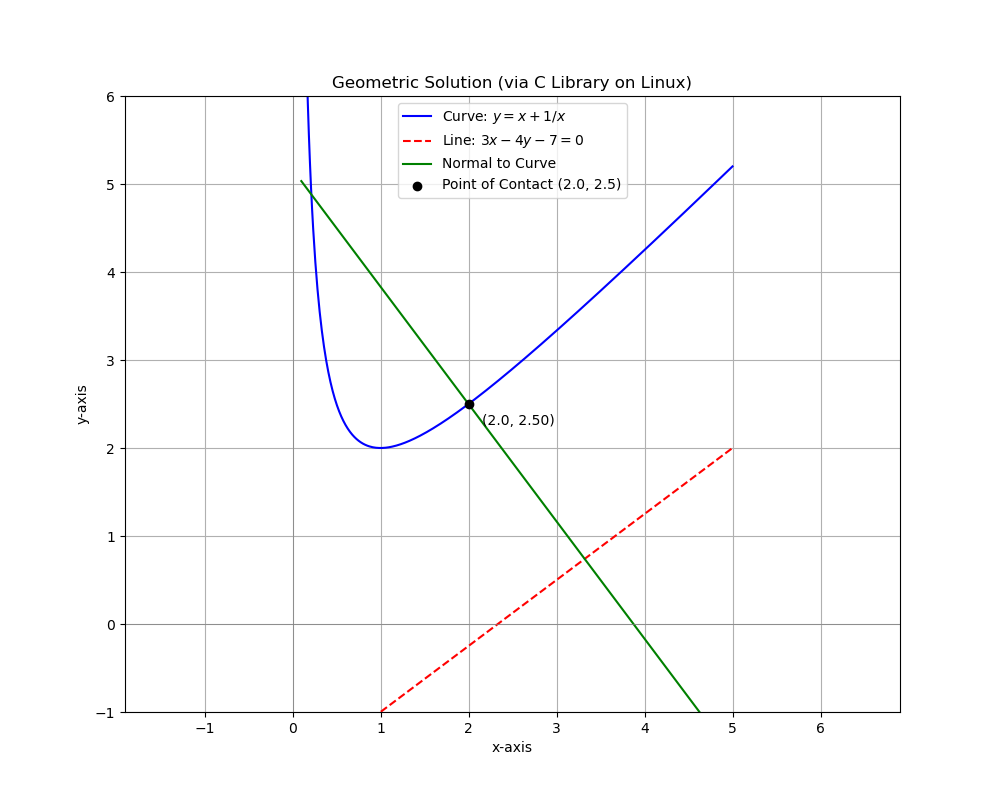
\includegraphics[width=\columnwidth, height=0.8\textheight, keepaspectratio]{figs/figure1.png}
        \end{center}
    \end{frame}
    
    \end{document}